\documentclass[11pt]{article}


\usepackage[left=1in, right=1in, top=1in, bottom=1in]{geometry}

\usepackage[style=chicago-authordate]{biblatex}
\usepackage{enumitem}

% Needed for the `modelsummary` TeX output from Rmd
\usepackage{tabularray}
\usepackage{float}
\usepackage{graphicx}

% \usepackage{codehigh}
% \usepackage[normalem]{ulem}
\UseTblrLibrary{booktabs}

\UseTblrLibrary{siunitx}
\newcommand{\tinytableTabularrayUnderline}[1]{\underline{#1}}
\newcommand{\tinytableTabularrayStrikeout}[1]{\sout{#1}}
\NewTableCommand{\tinytableDefineColor}[3]{\definecolor{#1}{#2}{#3}}

\usepackage{siunitx}
\usepackage{array}

\usepackage{amsmath}
\usepackage{amssymb}

\usepackage{multirow}

\usepackage{hyperref}

\addbibresource{references.bib}

\title{POLS 4724: Replication Experiment}
\author{Aman Choudhri}
\date{\today}

\begin{document}

\maketitle

In this paper, I replicate (and test for robustness to modeling choices)
the results of \cite{dymnickiAssessingImplementationEffects2021}. The original
paper is a 46 school randomized controlled trial of a holistic educational
intervention known as Safe Communities Safe Schools (SCSS). The SCSS program
was initiallly developed in 1999 at the University of Colorado Boulder's Center
for the Study and Prevention of Violence (CSPV) following the Columbine
shooting, with the goal of addressing mental/behavioral health concerns and
facilitating prosocial behavior. See \cite{SafeCommunitiesSafe} for more
information.

The variant of the program evaluated in
\cite{dymnickiAssessingImplementationEffects2021} consisted of three main components:
a team sited within each school dedicated to implementing the comprehensive program
over multiple years; ``capacity building'' to help school staff take advantage of data
in their decision-making; and the implementation of an evidence-based ``action plan''
to develop a school's support systems for students.

According to the authors,
this particular SCSS variant had previously not yet been evaluated in the literature.
They approach their experiment with the goals of studying how well the SCSS program is implemented,
as measured by qualitative rubric assessments from annual CSPV staff visits, and the effects
of the program on school climate, student behavior, and academic outcomes.

\section{Research Design}

The trial was conducted on $N = 46$ middle schools in Colorado, with a student
population of $S = 62590$ students. The study employed a staggered cohort
design with two cohorts ($N_{1} = 10, N_{2} = 36$) beginning one year apart.
Within each cohort, schools were matched into pairs based on school
characteristics and test scores, with one school from each pair randomly
assigned to either the treatment or waitlist control condition.

The evaluation followed schools over a three-year period (2016-2018),
with control schools scheduled to implement the treatment two years after their
cohort's treatment group began implementation. Due to the staggered nature of
the cohorts, the analysis focused on program effectiveness during the first two
years of implementation for each cohort to maintain comparability.

The key outcome variables of interest are:
\setlist{noitemsep}
\begin{itemize}
    \item \emph{School climate}, with subcategories like ``peer norms'' and ``violence
        indicators''. Climate was measured through annual student and staff
        surveys.
    \item \emph{Student behavior}, as measured by class attendance, truancy, and suspension rates.
        These data were obtained as school-level averages from the Colorado Department of Education.
    \item \emph{Student achievement}, as measured by math and reading standardized test scores. Again,
        the results were provided directly by the Colorado Department of Education.
\end{itemize}

\section{Replication and Robustness}

In this replication, we focus on studying outcome variables that are ``downstream''
of school climate—the more tangible phenomena of attendance,
truancy, suspensions, and academic achievement. Significant improvements on school climate,
which we might think of as a latent, amorphous construct, can reasonably be expected to manifest
in terms of these phenomena. So this restricted focus may still shed light on the main
social outcomes of interest to the SCSS program.

Unfortunately, baseline data for suspensions were not accessible through the public data
page, so the authors analyses of the impact of the program on that outcome variable
cannot be reproduced. So for behavioral outcomes, we analyze attendance and truancy only.

\subsection{Randomization Check}
Before proceeding with the replication, we first perform a randomization check
to assess whether treatment was effectively randomized within cohorts. The
randomization check is performed using by regressing the treatment indicator on
baseline school covariates (like the percentage of students eligible for free
or reduced price lunch) and the cohort indicator. See Table
\ref{table:school_summary_stats} for the full set of school-level covariates
examined, along with summary statistics for each.

The $F$-test test fails to reject the
null hypothesis of no correlation between covariate profiles and treatment with
$F = 0.531, p = 0.856$. As a result, we can be reasonably confident that the
randomization procedure was performed correctly and that there are no strange
inaccuracies from the matching process.

\subsection{School-Level Outcomes}
First, we match the paper and estimate the treatment effect on attendance and truancy.
The authors estimate two separate average treatment effects per
outcome variable: one after one year of treatment, and one after two years of treatment.
Following the paper's authors, we estimate each ATE
by pooling across the cohort groups and using a regression estimator:
\[
    Y_s^{(t)}  \sim \epsilon_s + \beta_{0}^{(t)}  + \beta_{1}^{(t)} Z_s + \beta_2^{(t)} y_s^{(0)} + X_s^T\beta_3 + \sum_{j = 2}^{23} \gamma_j I_{s \in \text{pair} \ i}
.\] 
In this notation, $Y_s ^{(t)}$ is the outcome variable for school $s$ in year $t$; $Z_s$ is of course
the treatment indicator; the variable
$y_s ^{(0)}$ represents the \emph{baseline} measurement of the outcome in the year prior to treatment;
$X_s$ is a matrix of the school-level covariates discussed in the previous section; and each $I_{s,i}$ is an indicator
variable representing whether school $s$ belongs to pair $i$.

All regression results accord with the analyses from the authors, finding no
treatment effects across the board. The coefficients, standard errors, and
p-values for the attendance and truancy outcome variables across years are
displayed in Table \ref{table:school_level_regressions}.

\begin{table}[htbp]
    \centering
    \caption{School-Level Outcome Treatment Effects}
    \vspace{0.4em}
    \label{table:school_level_regressions}
    \begin{tabular}{lccccccc}
    \toprule
    & & \multicolumn{3}{c}{Year 1} & \multicolumn{3}{c}{Year 2} \\
    \cmidrule(lr){3-5} \cmidrule(lr){6-8}
    Outcome & Model & $\beta^{(1)}$ & SE & $p$ & $\beta^{(2)}$ & SE & $p$ \\
    \midrule
    \multirow{2}{*}{Attendance} 
    & Original    & 0.010 & 0.0050 & 0.277 & 0.000 & 0.0050 & 0.949 \\
    & Replication & 0.006 & 0.0052 & 0.277 & 0.002 & 0.0050 & 0.697 \\
    \addlinespace[0.5em]
    \multirow{2}{*}{Truancy}    
    & Original    & 0.000 & 0.0040 & 0.261 & 0.000 & 0.0040 & 0.439 \\
    & Replication & -0.004 & 0.0038 & 0.261 & -0.005 & 0.0044 & 0.305 \\
    \bottomrule
    \multicolumn{6}{l}{\small Note: SE = standard error. Original results from \cite{dymnickiAssessingImplementationEffects2021}}
    \end{tabular}
\end{table}


An important methodological question is of missing data: one school closed down
during the experiment, leading to one complete missing row. Another school
became ``nonresponsive'' in the second year of the study. The authors removed
both schools and their pairs; if a significant treatment effect had emerged, it
may have been interesting to handle the attrition more carefully, especially
for the nonresponsive school. Since the findings are null, however, we proceed.

Both attendance and truancy having similarly null treatment effect findings does make sense,
since they largely capture the same phenomenon. It's interesting that the authors originally
chose to treat them as two separate outcomes, as Figure \ref{fig:attendance_vs_truancy} shows
quite a strong correlation between the two.

\begin{figure}[htbp]
    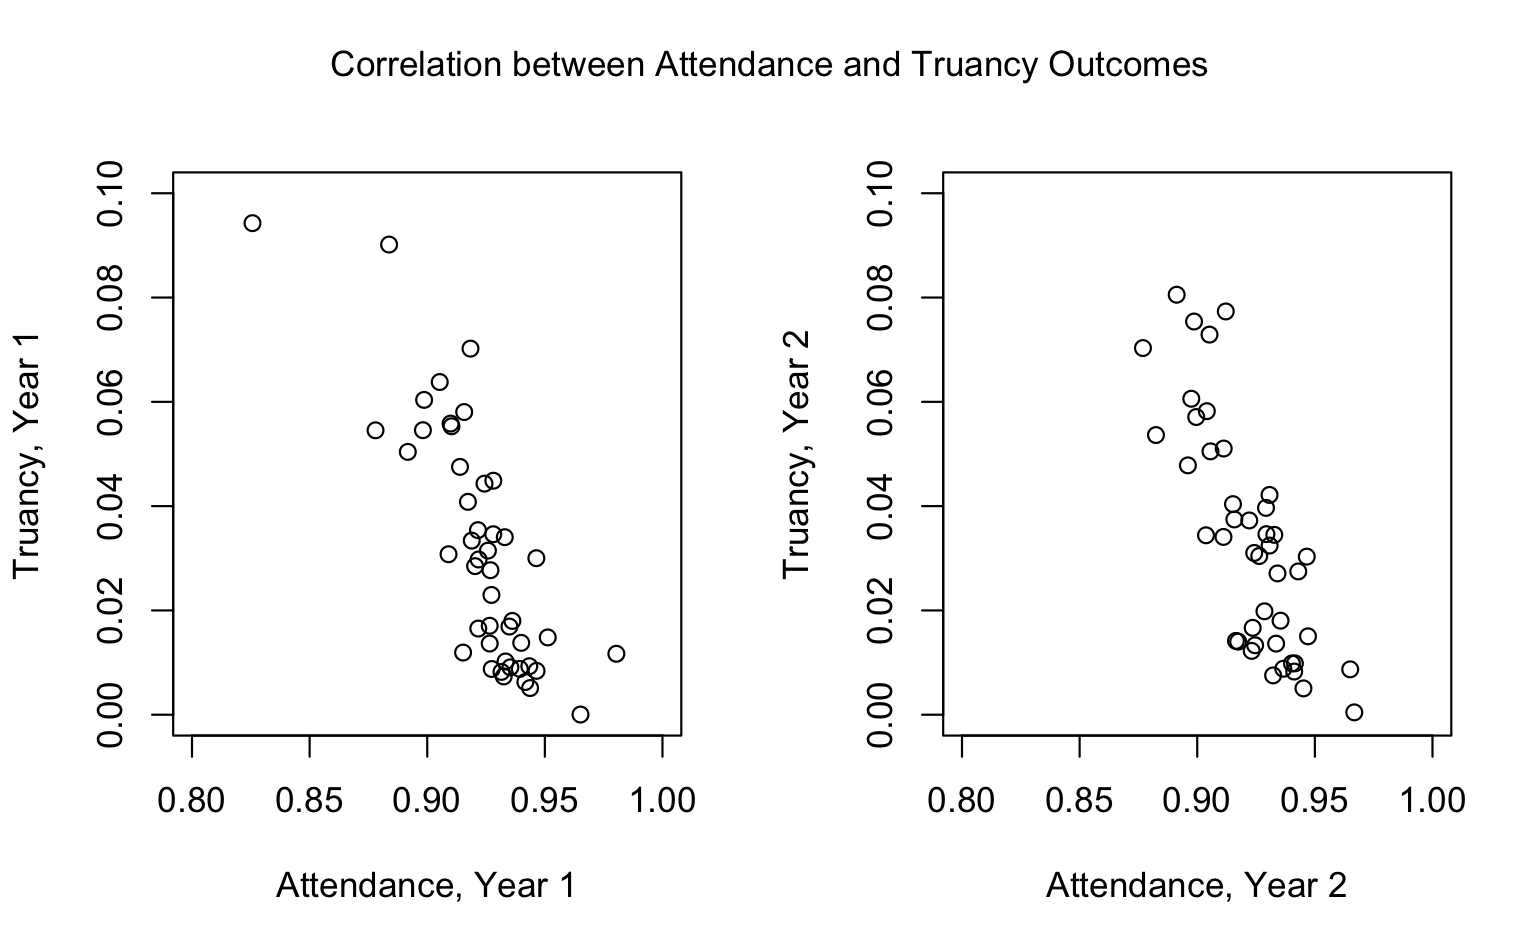
\includegraphics[scale=0.3]{img/attendance_vs_truancy.png}
    \caption{Relationship between Attendance and Truancy, by Treatment Year}
    \label{fig:attendance_vs_truancy}
\end{figure}

\subsection{Individual-Level Outcomes}
Next, we replicate the analysis of individual-level data on student
achievement. Achievement, in this context, is measured by standardized outcome
measures on state-wide reading and math examinations. The fact that the outcome
measures are standardized state-wide potentially poses an interesting spillover
effect violation. For a large enough sample size, it cannot be the case that
students in all schools have constant positive treatment effects. There are
$N_\text{population} = 289$ middle schools in Colorado, per the Department of
Education, meaning this experiment obtained outcome measurements from $N /
N_\text{population} = 15.9\%$ of all schools. This is a nontrivial fraction,
so it is worth keeping this fact about the outcome measurements in mind in the following
analysis.

Again, the authors estimate two separate treatment effects per outcome measure,
one for a one-year program treatment and one for a two-year treatment. Again, a
regression model is used, with baseline achievement scores used as
individual-level covariates.

The authors also include individual-level
demographic information as covariates, many of which have been redacted in the
public dataset. We estimate a model using only the available covariates
(Male/Female, White/Non-White) to understand the sensitivity of the treatment
effect estimate to the model specification.

The results from the regressions are shown in Table
\ref{tab:academic-achievement}. In general, the results are similar. Effect sizes
are generally near to the original paper's. However, the obtained standard errors
under these modeling choices are \emph{far} higher in general. In fact, the standard
errors can be so large as to render findings that were significant under the original
paper insignificant.

This pattern is potentially due to the lack of individual-level
covariates: the original model's additional demographic covariates may have helped explain
variation in test scores, leading to tighter estimates. By contrast,
our model may be running into an identification issue with too many degrees of freedom relative to the effective sample size.
Without individual covariates to help explain variability within schools, the
model might be struggling to separate different sources of variation.

\begin{table}[htbp]
    \centering
    \caption{Effects on Reading and Math Academic Achievement Test Scores}
    \label{tab:academic-achievement}
    \begin{tabular}{lllccccccc}
    \toprule
    & & & \multicolumn{3}{c}{Year 1} & \multicolumn{3}{c}{Year 2} \\
    \cmidrule(lr){4-6} \cmidrule(lr){7-9}
    Outcome & Grade & Model & $\beta$ & SE & $p$ & $\beta$ & SE & $p$ \\
    \midrule
    \multirow{4}{*}{Reading} & \multirow{2}{*}{7} 
    & Original    & 0.10 & 0.021 & 0.000 & -- & -- & -- \\
    & & Replication & 0.176 & 0.0560 & 0.00274 & -- & -- & -- \\
    \addlinespace[0.3em]
    & \multirow{2}{*}{8} 
    & Original    & 0.12 & 0.023 & 0.000 & 0.11 & 0.025 & 0.000 \\
    & & Replication & 0.142 & 0.0723 & 0.0697 & 0.092 & 0.070 & 0.2231 \\
    \midrule
    \multirow{4}{*}{Math} & \multirow{2}{*}{7}
    & Original    & 0.03 & 0.020 & 0.076 & -- & -- & -- \\
    & & Replication & 0.032 & 0.0343 & 0.371 & -- & -- & -- \\
    \addlinespace[0.3em]
    & \multirow{2}{*}{8}
    & Original    & -0.01 & 0.027 & 0.739 & 0.01 & 0.024 & 0.795 \\
    & & Replication & -0.007 & 0.0050 & 0.8887 & 0.00129 & 0.0573 & 0.9823  \\
    \bottomrule
    \multicolumn{9}{l}{\small Note: SE = standard error. Original results from \cite{dymnickiAssessingImplementationEffects2021}}
    \end{tabular}
\end{table}

\subsection{Robustness Check: Other Modeling Approaches}

To attempt to repair the precision problem with the model we specified, we now
attempt a different model specification. This has the two-fold benefit of 1)
probing whether the large standard errors can be repaired, and 2) understanding
the extent to which estimated treatment effects are robust to other sensible
modeling choices.

Rather than fitting two separate models for each grade level to estimate one-year
treatment effects, we now
try pooling data across grades while
allowing for grade-specific treatment effects through interaction terms. This
approach increases statistical power by sharing information across grades while
still allowing for different treatment effects.

The results are displayed in Table \ref{tab:pooled-interact-results}. We observe
notably precise treatment effects than our
previous specifications. For reading scores, we find large positive effects in both
grades: about 0.21 points in Grade 7 (p $<$ 0.001) and 0.15 
in Grade 8 (p = 0.002). These estimates are not only more precise
than our previous replication attempts but also suggest larger effects than the
original paper reported.

The math results show an interesting pattern of effect heterogeneity: while
Grade 7 shows no effect (in accordance with the previous replication and
original results), Grade 8 shows a modest positive effect of 0.065 standard
deviations (p = 0.024). This
grade-level heterogeneity in math impacts was masked in the previous
specifications, highlighting the value of this modeling approach in uncovering
nuanced treatment effects.

\begin{table}[htbp]
\centering
\caption{One-Year Treatment Effects by Grade Level (Interaction Model)}
\label{tab:pooled-interact-results}
\begin{tabular}{llcccccc}
\toprule
& & & & & \multicolumn{2}{c}{Sample} \\
\cmidrule(lr){6-7}
Outcome & Grade & $\beta$ & SE & $p$-value & $N$ & \% Treated \\
\midrule
\multirow{2}{*}{Reading} 
& 7 & 0.215 & 0.046 & $<$0.001 & 3,789 & 63.9\% \\
& 8 & 0.150 & 0.047 & 0.002 & 3,513 & 64.9\% \\
\addlinespace[0.5em]
\multirow{2}{*}{Math}    
& 7 & -0.012 & 0.025 & 0.636 & 3,789 & 63.9\% \\
& 8 & 0.065 & 0.026 & 0.024 & 3,513 & 64.9\% \\
\bottomrule
\multicolumn{7}{l}{\small Note: Results from pooled model with treatment-by-grade interactions.} \\
\end{tabular}
\end{table}

\section{Conclusion}

The replication effort yielded mixed but instructive results. For school-level
outcomes like attendance and truancy, our analysis closely matched the original
findings, confirming null effects across both treatment years. However, our
attempt to replicate the student achievement analysis revealed the crucial role
of modeling choices and data availability in treatment effect estimation.

The original achievement analysis relied on individual-level demographic
covariates that were redacted in the public dataset. Our initial replication
attempt, using only available covariates, produced similar point estimates but
with substantially larger standard errors, making some previously significant
effects statistically insignificant. This highlighted how omitted
individual-level controls, while not necessarily biasing treatment effect
estimates, can reduce precision and blur the lines of statistical significance.

However, adopting a different modeling approach that pooled information
across grades while allowing for heterogeneous treatment effects yielded
notably different results. This specification not only improved precision but
also uncovered potentially larger—but also potentially implausible—treatment
effects in reading. The contrast between these results and both the original paper and our first
replication attempt underscores just how important methodological choices can be when
analyzing even data from a randomized experiment.

\section*{Data and Code Availability}
All code used for this replication is available at
\url{https://github.com/amanchoudhri/scss-replication/tree/main}. The
repository includes the full replication code and documentation of the analysis
workflow.

\printbibliography

\appendix

\section{School Covariate Summary Statistics}

\begin{table}[h]
\centering
\begin{talltblr}[         %% tabularray outer open
caption={School-Level Covariate Summary Statistics},
]                     %% tabularray outer close
{                     %% tabularray inner open
colspec={Q[]Q[]Q[]},
column{1}={}{halign=l,},
column{2,3}={}{halign=r,},
}                     %% tabularray inner close
\toprule
& Mean & Std. Dev. \\ \midrule %% TinyTableHeader
Proportion Eligible for Free/Reduced Lunch        & \num{0.596}  & \num{0.277}  \\
Student-Teacher Ratio                             & \num{16.008} & \num{3.303}  \\
\% Black                                         & \num{7.318}  & \num{9.763}  \\
\% Hispanic                                      & \num{47.564} & \num{28.692} \\
\% White                                         & \num{37.901} & \num{29.858} \\
Small 6th and 7th Grades (less than 200 students) & \num{0.304}  & \num{0.465}  \\
Large 6th and 7th Grades (more than 700 students) & \num{0.196}  & \num{0.401}  \\
Also an Elementary School                         & \num{0.261}  & \num{0.444}  \\
Also a High School                                & \num{0.087}  & \num{0.285}  \\
\bottomrule
\end{talltblr}
\label{table:school_summary_stats}
\end{table}


\end{document}
